\documentclass{beamer} 
\usepackage[english]{babel}
\usepackage{graphicx}
\usepackage{color}
\usepackage{verbatim}
\usepackage{bm}
\usepackage{ulem}
\usepackage{amsfonts}
\usepackage{pgf}
\usepackage{textpos}


%%%%R commands for running Sweave%%%%%%%
%%%%setwd("/users/stevenwalker/documents/presentations/concordiaseminar/bilinear/")
%%%%Sweave("/users/stevenwalker/documents/presentations/concordiaseminar/bilinear/bilinear.Rnw")


\setbeamertemplate{blocks}[rounded]
%\setbeamercolor{frametitle}{fg=red} 

\usetheme{Goettingen}
\usecolortheme{rose}
%\useoutertheme{infolines} 
\usecolortheme{seahorse} 

\pgfdeclareimage[height=0.7cm]{logo}{uni_logo} 
\logo{\pgfuseimage{logo}} 

\title[Data management]{Predicting community composition using site and species characteristics:  a data management perspective}
\author[Steve C. Walker \\ Guillaume Gu\'{e}nard \\ Pierre Legendre]{Steve C. Walker, Guillaume Gu\'{e}nard, and Pierre Legendre} 
\institute[Montr\'{e}al]{\insertlogo \\ D\'{e}partement de Sciences Biologiques}
\date[August 12, 2011]{August 12, 2011 \\ Ecological Society of America \\ Austin, Texas}

\usepackage{url}
\usepackage{amssymb}
\usepackage{amsmath}  

%\newcommand{\R}{{\sf R}}
\newcommand{\code}[1]{\texttt{#1}}


\newcounter{exercise}
\numberwithin{exercise}{section}
\newcommand{\exnumber}{\addtocounter{exercise}{1} \theexercise \thinspace}

\newcommand{\R}{
\includegraphics[width=0.5cm]{Rlogo}}

%\usepackage{Sweave}
\begin{document}
\maketitle

\section{Introduction}

\subsection[Traits and ecology]{Traits and the ecology of communities}
\frame{\tableofcontents[currentsection,currentsubsection]}

%%%%%
\begin{frame}
\frametitle{\textit{Bythotrephes longimanus}}
\begin{center}
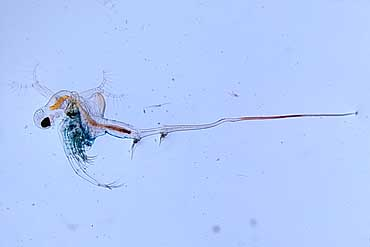
\includegraphics[width=8cm]{waterflea}
\end{center}
\vspace{0.5cm}
\footnotesize{Wisconsin Department of Natural Resources}
\end{frame}
%%%%%

%%%%%
\begin{frame}
\frametitle{\textit{Bythotrephes longimanus}}
\begin{center}
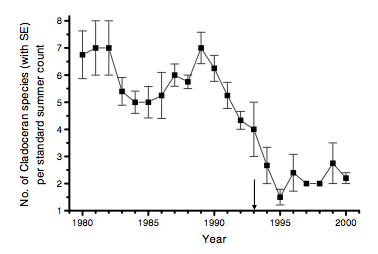
\includegraphics[width=8cm]{Yan}
\end{center}
\vspace{0.5cm}
\footnotesize{Yan et al. (2002)}
\end{frame}
%%%%%

\subsection{Illustrative example}
\frame{\tableofcontents[currentsection,currentsubsection]}

\begin{frame}
\frametitle{Fourth corner}
\small
% latex table generated in R 2.10.1 by xtable 1.5-6 package
% Tue Feb  8 08:19:58 2011
\begin{table}[ht]
\begin{center}
\begin{tabular}{r|rrrr|r|}
  & sp 1 & sp 2 & sp 3 & sp 4 \\ 
  \hline
site 1 & 0.1 & 2.1 & 0.1 & 1.5  \\ 
  site 2 & 0.7 & -0.9 & 1.8 & 3.7  \\ 
  site 3 & 1.1 & 0.5 & 1.5 & 2.8  \\ 
  site 4 & 1.3 & -2.0 & 3.0 & -0.2  \\ 
  site 5 & 1.7 & 2.0 & 1.3 & 1.2  \\ 
  site 6 & 0.8 & -0.1 & 2.0 & 1.1  \\ 
  site 7 & -2.6 & -1.4 & 1.8 & 4.1  \\ 
  site 8 & -0.0 & 1.5 & 2.3 & 2.3  \\ 
   \hline
\end{tabular}
\end{center}
\end{table}\normalsize
\end{frame}

\begin{frame}
\frametitle{Fourth corner}
\small
% latex table generated in R 2.10.1 by xtable 1.5-6 package
% Tue Feb  8 08:19:58 2011
\begin{table}[ht]
\begin{center}
\begin{tabular}{r|rrrr|r|}
  & sp 1 & sp 2 & sp 3 & sp 4 & environment \\ 
  \hline
site 1 & 0.1 & 2.1 & 0.1 & 1.5 & -0.3 \\ 
  site 2 & 0.7 & -0.9 & 1.8 & 3.7 & 1.4 \\ 
  site 3 & 1.1 & 0.5 & 1.5 & 2.8 & -0.1 \\ 
  site 4 & 1.3 & -2.0 & 3.0 & -0.2 & 0.4 \\ 
  site 5 & 1.7 & 2.0 & 1.3 & 1.2 & -0.3 \\ 
  site 6 & 0.8 & -0.1 & 2.0 & 1.1 & -0.6 \\ 
  site 7 & -2.6 & -1.4 & 1.8 & 4.1 & 2.0 \\ 
  site 8 & -0.0 & 1.5 & 2.3 & 2.3 & 0.7 \\ 
   \hline
\end{tabular}
\end{center}
\end{table}\normalsize
\end{frame}

\begin{frame}
\frametitle{Fourth corner}
\small
% latex table generated in R 2.10.1 by xtable 1.5-6 package
% Tue Feb  8 08:19:58 2011
\begin{table}[ht]
\begin{center}
\begin{tabular}{r|rrrr|r|}
  & sp 1 & sp 2 & sp 3 & sp 4 & environment \\ 
  \hline
site 1 & 0.1 & 2.1 & 0.1 & 1.5 & -0.3 \\ 
  site 2 & 0.7 & -0.9 & 1.8 & 3.7 & 1.4 \\ 
  site 3 & 1.1 & 0.5 & 1.5 & 2.8 & -0.1 \\ 
  site 4 & 1.3 & -2.0 & 3.0 & -0.2 & 0.4 \\ 
  site 5 & 1.7 & 2.0 & 1.3 & 1.2 & -0.3 \\ 
  site 6 & 0.8 & -0.1 & 2.0 & 1.1 & -0.6 \\ 
  site 7 & -2.6 & -1.4 & 1.8 & 4.1 & 2.0 \\ 
  site 8 & -0.0 & 1.5 & 2.3 & 2.3 & 0.7 \\ 
   \hline
  trait & -1.0 & -1.0 & 1.0 & 1.0 &  \\ 
   \hline
\end{tabular}
\end{center}
\end{table}\normalsize 
\end{frame}

\begin{frame}
\frametitle{Fourth corner}
\small
% latex table generated in R 2.10.1 by xtable 1.5-6 package
% Tue Feb  8 08:19:58 2011
\begin{table}[ht]
\begin{center}
\begin{tabular}{r|rrrr|r|}
  & sp 1 & sp 2 & sp 3 & sp 4 & environment \\ 
  \hline
site 1 & 0.1 & 2.1 & 0.1 & 1.5 & -0.3 \\ 
  site 2 & 0.7 & -0.9 & 1.8 & 3.7 & 1.4 \\ 
  site 3 & 1.1 & 0.5 & 1.5 & 2.8 & -0.1 \\ 
  site 4 & 1.3 & -2.0 & 3.0 & -0.2 & 0.4 \\ 
  site 5 & 1.7 & 2.0 & 1.3 & 1.2 & -0.3 \\ 
  site 6 & 0.8 & -0.1 & 2.0 & 1.1 & -0.6 \\ 
  site 7 & -2.6 & -1.4 & 1.8 & 4.1 & 2.0 \\ 
  site 8 & -0.0 & 1.5 & 2.3 & 2.3 & 0.7 \\ 
   \hline
  trait & -1.0 & -1.0 & 1.0 & 1.0 & \textcolor{red}{\textbf{??}} \\ 
   \hline
\end{tabular}
\end{center}
\end{table}\normalsize 
\begin{textblock}{100}(10.2,-0.5)
\textcolor{red}{$\mathbf{\uparrow}$}
\end{textblock}
\begin{textblock}{100}(11,-1.25)
\textcolor{red}{$\mathbf{\leftarrow}$}
\end{textblock}
\begin{textblock}{100}(9.3,-1.25)
\textcolor{red}{$\mathbf{\rightarrow}$}
\end{textblock}
\end{frame}

\subsection{Complex example}
\frame{\tableofcontents[currentsection,currentsubsection]}



\subsection{Data management}
\frame{\tableofcontents[currentsection,currentsubsection]}

\begin{frame}
\frametitle{Linear algebra as data management}
\begin{center}
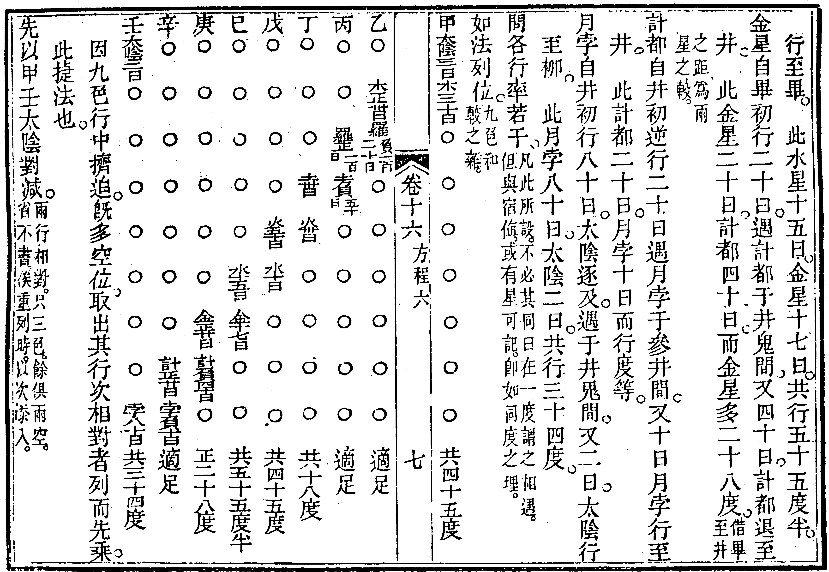
\includegraphics[scale=0.6]{fangcheng}
\end{center}
%\vspace{0.5cm}
\footnotesize{Ancient Chinese text ($\sim$150 BCE)}
\end{frame}

\begin{frame}
\frametitle{Linear algebra as data management}
\begin{center}
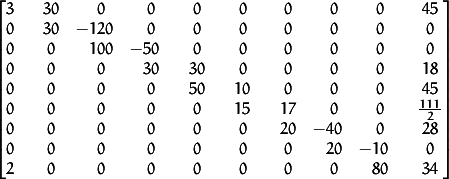
\includegraphics[scale=0.6]{fangchengmodern}
\end{center}
%\vspace{0.5cm}
\footnotesize{Hart (2009)}
\end{frame}

\begin{frame}
\frametitle{Linear algebra as data management}
\begin{center}
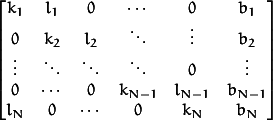
\includegraphics[scale=0.6]{fangchengmoderngeneral}
\end{center}
%\vspace{0.5cm}
\footnotesize{Hart (2009)}
\end{frame}

\begin{frame}
\frametitle{Linear algebra as data management}
\begin{center}
\begin{equation}
\begin{split}
\mathbf{Y} &= \mathbf{XB} \\
\uncover<2->{\mathbf{X^{T}Y} &= \mathbf{X^{T}XB}} \\
\uncover<3->{\mathbf{(X^{T}X)}^{-1}\mathbf{X^{T}Y} &= \mathbf{B}} \\
\end{split}
\end{equation}
\end{center}
\end{frame}

\begin{frame}
\frametitle{The R paradigm of data management}
\begin{center}
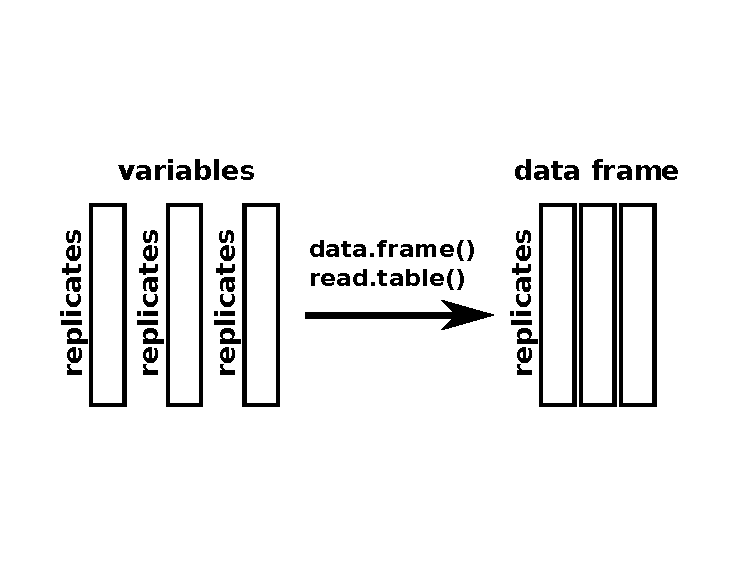
\includegraphics[scale=0.6]{vectors2dataframe}
\end{center}
\end{frame}

\begin{frame}
\frametitle{The R paradigm of data management}
\begin{center}
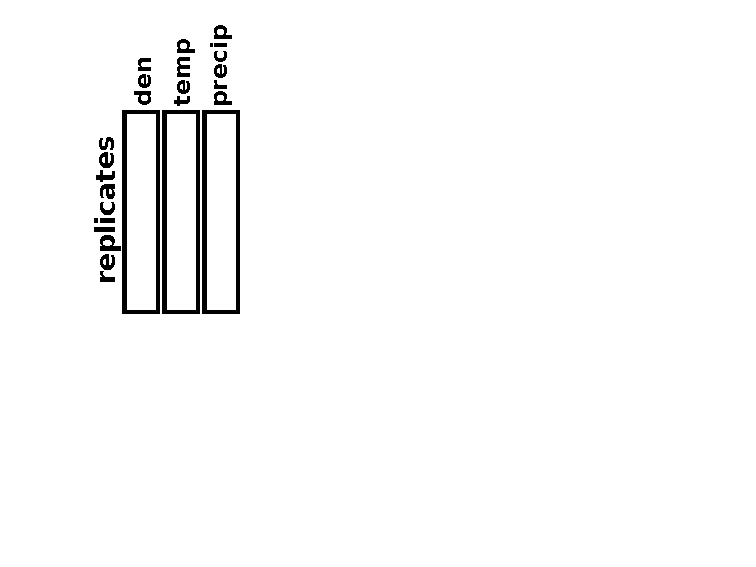
\includegraphics[scale=0.6]{dataframe2function1}
\end{center}
\end{frame}

\begin{frame}
\frametitle{The R paradigm of data management}
\begin{center}
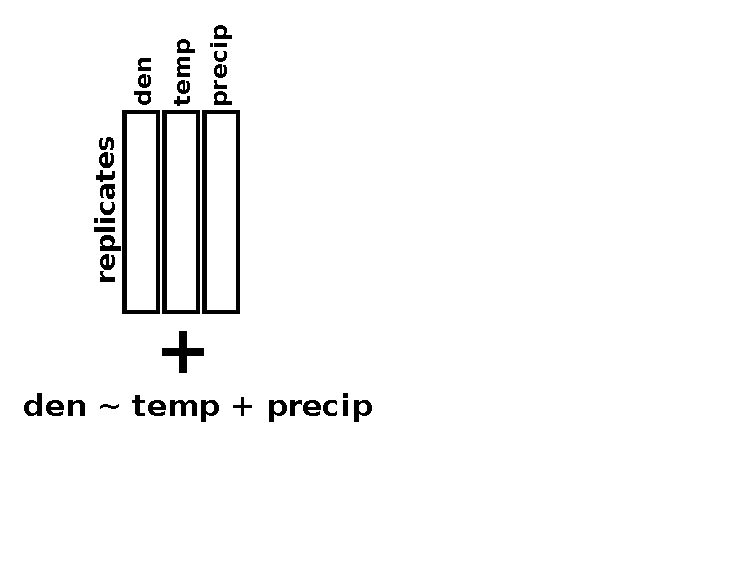
\includegraphics[scale=0.6]{dataframe2function2}
\end{center}
\end{frame}

\begin{frame}
\frametitle{The R paradigm of data management}
\begin{center}
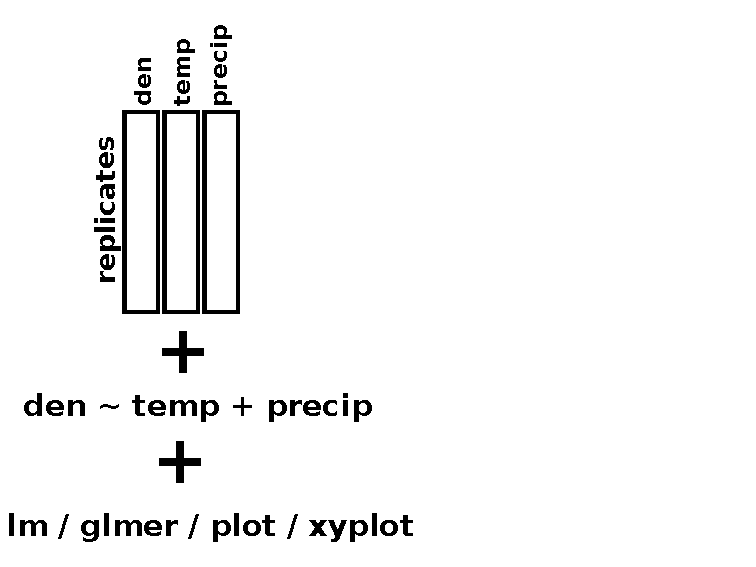
\includegraphics[scale=0.6]{dataframe2function3}
\end{center}
\end{frame}

\begin{frame}
\frametitle{The R paradigm of data management}
\begin{center}
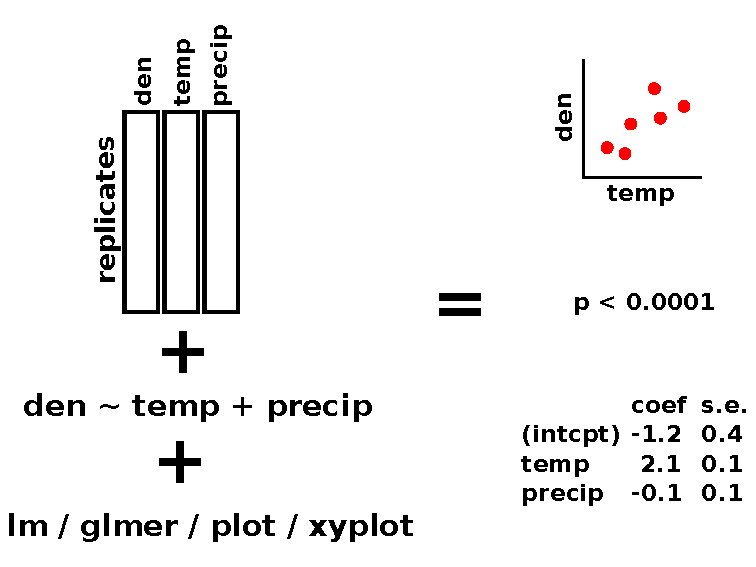
\includegraphics[scale=0.6]{dataframe2function4}
\end{center}
\end{frame}

\setlength{\tabcolsep}{2.5pt}
\begin{frame}
\frametitle{The R paradigm of data management}
\begin{center}
\begin{tabular}{ccccccc}
DATA FRAME&+&FORMULA&+&FUNCTION&=&ANALYSIS \\
\\
\end{tabular}
\end{center}
\end{frame}
\setlength{\tabcolsep}{6pt}

\setlength{\tabcolsep}{2.5pt}
\begin{frame}
\frametitle{The R paradigm of data management}
\begin{center}
\begin{tabular}{ccccccc}
\textbf{DATA FRAME}&+&FORMULA&+&FUNCTION&=&ANALYSIS \\
data management \\
\end{tabular}
\end{center}
\end{frame}
\setlength{\tabcolsep}{6pt}

\setlength{\tabcolsep}{2.5pt}
\begin{frame}
\frametitle{The R paradigm of data management}
\begin{center}
\begin{tabular}{ccccccc}
DATA FRAME&+&\textbf{FORMULA}&+&FUNCTION&=&ANALYSIS \\
&&ecological ideas \\
\end{tabular}
\end{center}
\end{frame}
\setlength{\tabcolsep}{6pt}

\setlength{\tabcolsep}{2.5pt}
\begin{frame}
\frametitle{The R paradigm of data management}
\begin{center}
\begin{tabular}{ccccccc}
DATA FRAME&+&FORMULA&+&\textbf{FUNCTION}&=&ANALYSIS \\
&&&&algorithms \\
\end{tabular}
\end{center}
\end{frame}
\setlength{\tabcolsep}{6pt}

\setlength{\tabcolsep}{2.5pt}
\begin{frame}
\frametitle{The R paradigm of data management}
\begin{center}
\begin{tabular}{ccccccc}
DATA FRAME&+&FORMULA&+&FUNCTION&=&\textbf{ANALYSIS} \\
 \\
\end{tabular}
\end{center}
\end{frame}
\setlength{\tabcolsep}{6pt}

\section{Methods}

\section{Results}

\begin{comment}

%%%%%
\begin{frame}
\frametitle{Traits et phylog\'{e}nies}
\begin{center}
\includegraphics[width=4cm]{phylogeny}
\end{center}
\footnotesize{Cavender-Bares et al. (2009)}
\end{frame}
%%%%%

%%%%%
\begin{frame}
\frametitle{Tests d'hypoth\`{e}se}
\begin{center}
\includegraphics[width=6cm]{pillar}
\end{center}
\vspace{-0.5cm}
\footnotesize{Pillar and Duarte (2010)}
\end{frame}
%%%%%

%%%%%
\begin{frame}
\frametitle{Rarement utilis\'{e}s pour pr\'{e}dire}
\begin{center}
\includegraphics[width=6cm]{Ives}
\end{center}
\vspace{-0.5cm}
\footnotesize{Ives and Godrey (2006)}
\end{frame}
%%%%%

\subsection{Exemple illustratif}
\frame{\tableofcontents[currentsection,currentsubsection]}

\begin{frame}
\frametitle{Quatri\`{e}me coin}
\small
% latex table generated in R 2.10.1 by xtable 1.5-6 package
% Tue Feb  8 08:19:58 2011
\begin{table}[ht]
\begin{center}
\begin{tabular}{r|rrrr|r|}
  & sp 1 & sp 2 & sp 3 & sp 4 \\ 
  \hline
site 1 & 0.1 & 2.1 & 0.1 & 1.5  \\ 
  site 2 & 0.7 & -0.9 & 1.8 & 3.7  \\ 
  site 3 & 1.1 & 0.5 & 1.5 & 2.8  \\ 
  site 4 & 1.3 & -2.0 & 3.0 & -0.2  \\ 
  site 5 & 1.7 & 2.0 & 1.3 & 1.2  \\ 
  site 6 & 0.8 & -0.1 & 2.0 & 1.1  \\ 
  site 7 & -2.6 & -1.4 & 1.8 & 4.1  \\ 
  site 8 & -0.0 & 1.5 & 2.3 & 2.3  \\ 
   \hline
\end{tabular}
\end{center}
\end{table}\normalsize
\end{frame}

\begin{frame}
\frametitle{Quatri\`{e}me coin}
\small
% latex table generated in R 2.10.1 by xtable 1.5-6 package
% Tue Feb  8 08:19:58 2011
\begin{table}[ht]
\begin{center}
\begin{tabular}{r|rrrr|r|}
  & sp 1 & sp 2 & sp 3 & sp 4 & environment \\ 
  \hline
site 1 & 0.1 & 2.1 & 0.1 & 1.5 & -0.3 \\ 
  site 2 & 0.7 & -0.9 & 1.8 & 3.7 & 1.4 \\ 
  site 3 & 1.1 & 0.5 & 1.5 & 2.8 & -0.1 \\ 
  site 4 & 1.3 & -2.0 & 3.0 & -0.2 & 0.4 \\ 
  site 5 & 1.7 & 2.0 & 1.3 & 1.2 & -0.3 \\ 
  site 6 & 0.8 & -0.1 & 2.0 & 1.1 & -0.6 \\ 
  site 7 & -2.6 & -1.4 & 1.8 & 4.1 & 2.0 \\ 
  site 8 & -0.0 & 1.5 & 2.3 & 2.3 & 0.7 \\ 
   \hline
\end{tabular}
\end{center}
\end{table}\normalsize
\end{frame}

\begin{frame}
\frametitle{Quatri\`{e}me coin}
\small
% latex table generated in R 2.10.1 by xtable 1.5-6 package
% Tue Feb  8 08:19:58 2011
\begin{table}[ht]
\begin{center}
\begin{tabular}{r|rrrr|r|}
  & sp 1 & sp 2 & sp 3 & sp 4 & environment \\ 
  \hline
site 1 & 0.1 & 2.1 & 0.1 & 1.5 & -0.3 \\ 
  site 2 & 0.7 & -0.9 & 1.8 & 3.7 & 1.4 \\ 
  site 3 & 1.1 & 0.5 & 1.5 & 2.8 & -0.1 \\ 
  site 4 & 1.3 & -2.0 & 3.0 & -0.2 & 0.4 \\ 
  site 5 & 1.7 & 2.0 & 1.3 & 1.2 & -0.3 \\ 
  site 6 & 0.8 & -0.1 & 2.0 & 1.1 & -0.6 \\ 
  site 7 & -2.6 & -1.4 & 1.8 & 4.1 & 2.0 \\ 
  site 8 & -0.0 & 1.5 & 2.3 & 2.3 & 0.7 \\ 
   \hline
  trait & -1.0 & -1.0 & 1.0 & 1.0 & 0.8 \\ 
   \hline
\end{tabular}
\end{center}
\end{table}\normalsize 
\end{frame}

\begin{frame}
\frametitle{Quatri\`{e}me coin}
\small
% latex table generated in R 2.10.1 by xtable 1.5-6 package
% Tue Feb  8 08:19:58 2011
\begin{table}[ht]
\begin{center}
\begin{tabular}{r|rrrr|r|}
  & sp 1 & sp 2 & sp 3 & sp 4 & environment \\ 
  \hline
site 1 & 0.1 & 2.1 & 0.1 & 1.5 & -0.3 \\ 
  site 2 & 0.7 & -0.9 & 1.8 & 3.7 & 1.4 \\ 
  site 3 & 1.1 & 0.5 & 1.5 & 2.8 & -0.1 \\ 
  site 4 & 1.3 & -2.0 & 3.0 & -0.2 & 0.4 \\ 
  site 5 & 1.7 & 2.0 & 1.3 & 1.2 & -0.3 \\ 
  site 6 & 0.8 & -0.1 & 2.0 & 1.1 & -0.6 \\ 
  site 7 & -2.6 & -1.4 & 1.8 & 4.1 & 2.0 \\ 
  site 8 & -0.0 & 1.5 & 2.3 & 2.3 & 0.7 \\ 
   \hline
  trait & -1.0 & -1.0 & 1.0 & 1.0 & 0.8 \\ 
   \hline
\end{tabular}
\end{center}
\end{table}\normalsize 
\begin{textblock}{100}(10.2,-0.5)
$\uparrow$
\end{textblock}
\begin{textblock}{100}(11,-1.25)
$\leftarrow$
\end{textblock}
\begin{textblock}{100}(9.3,-1.25)
$\rightarrow$
\end{textblock}
\end{frame}

\begin{frame}
\frametitle{Quatri\`{e}me coin}
\small
% latex table generated in R 2.10.1 by xtable 1.5-6 package
% Tue Feb  8 08:19:58 2011
\begin{table}[ht]
\begin{center}
\begin{tabular}{r|rrrr|rr|}
  & sp 1 & sp 2 & sp 3 & sp 4 & intercept & environment \\ 
  \hline
site 1 & 0.1 & 2.1 & 0.1 & 1.5 & 1.0 & -0.3 \\ 
  site 2 & 0.7 & -0.9 & 1.8 & 3.7 & 1.0 & 1.4 \\ 
  site 3 & 1.1 & 0.5 & 1.5 & 2.8 & 1.0 & -0.1 \\ 
  site 4 & 1.3 & -2.0 & 3.0 & -0.2 & 1.0 & 0.4 \\ 
  site 5 & 1.7 & 2.0 & 1.3 & 1.2 & 1.0 & -0.3 \\ 
  site 6 & 0.8 & -0.1 & 2.0 & 1.1 & 1.0 & -0.6 \\ 
  site 7 & -2.6 & -1.4 & 1.8 & 4.1 & 1.0 & 2.0 \\ 
  site 8 & -0.0 & 1.5 & 2.3 & 2.3 & 1.0 & 0.7 \\ 
   \hline
intercept & 1.0 & 1.0 & 1.0 & 1.0 & 1.2 & -0.2 \\ 
  trait & -1.0 & -1.0 & 1.0 & 1.0 & 0.5 & 0.8 \\ 
   \hline
\end{tabular}
\end{center}
\end{table}\normalsize
\end{frame}


\begin{frame}
\begin{center}
\begin{figure}
\includegraphics{bilinear-005}
\end{figure}
\end{center}
\end{frame}

\begin{frame}[fragile]
\begin{center}
\begin{Schunk}
\begin{Soutput}
            intercept trait
intercept        1.15  0.46
environment     -0.15  0.84
\end{Soutput}
\end{Schunk}
\begin{figure}
\includegraphics{bilinear-007}
\end{figure}
\end{center}
\end{frame}

\section{Mod\`{e}les bilin\'{e}aires}

\subsection[Quatri\`{e}me coin]{Solution bilin\'{e}aire au probl\`{e}me du quatri\`{e}me coin}
\frame{\tableofcontents[currentsection,currentsubsection]}

\begin{frame}
\frametitle{Quatri\`{e}me coin}
\small
% latex table generated in R 2.10.1 by xtable 1.5-6 package
% Tue Feb  8 08:19:58 2011
\begin{table}[ht]
\begin{center}
\begin{tabular}{r|rrrr|rr|}
  & sp 1 & sp 2 & sp 3 & sp 4 & intercept & environment \\ 
  \hline
site 1 & 0.1 & 2.1 & 0.1 & 1.5 & 1.0 & -0.3 \\ 
  site 2 & 0.7 & -0.9 & 1.8 & 3.7 & 1.0 & 1.4 \\ 
  site 3 & 1.1 & 0.5 & 1.5 & 2.8 & 1.0 & -0.1 \\ 
  site 4 & 1.3 & -2.0 & 3.0 & -0.2 & 1.0 & 0.4 \\ 
  site 5 & 1.7 & 2.0 & 1.3 & 1.2 & 1.0 & -0.3 \\ 
  site 6 & 0.8 & -0.1 & 2.0 & 1.1 & 1.0 & -0.6 \\ 
  site 7 & -2.6 & -1.4 & 1.8 & 4.1 & 1.0 & 2.0 \\ 
  site 8 & -0.0 & 1.5 & 2.3 & 2.3 & 1.0 & 0.7 \\ 
   \hline
intercept & 1.0 & 1.0 & 1.0 & 1.0 & 1.2 & -0.2 \\ 
  trait & -1.0 & -1.0 & 1.0 & 1.0 & 0.5 & 0.8 \\ 
   \hline
\end{tabular}
\end{center}
\end{table}\normalsize
\end{frame}

\begin{frame}
\frametitle{Quatri\`{e}me coin}
\begin{center}
\includegraphics[width=5cm]{fourthcornerfigure.pdf}
\end{center}
\end{frame}

\begin{frame}
\begin{block}{D\'{e}finitions}
Variables: $y$ (communaut\'{e}), $x$ (environnement), $z$ (les traits) \\
\pause
Indices: $i$ (site), $j$ (esp\`{e}ces), $k$ (var. env.), $l$ (trait)
\pause
\end{block}
\begin{block}{Mod\`{e}le lin\'{e}aire}
\begin{equation}
\begin{gathered}
y_{ij} = \sum_{k=1}^{p} x_{ik}b_{kj} + e_{ij} \\
%\mathbf{Y} = \mathbf{XB} + \mathbf{E}
%\pause
\end{gathered}
\end{equation}
\end{block}
\pause
\begin{block}{Mod\`{e}le bilin\'{e}aire}
\begin{equation}
\begin{gathered}
y_{ij} = \sum_{k=1}^{p} \sum_{l=1}^{q} x_{ik}z_{jl}c_{kl} + e_{ij} \\
%\pause
%\mathbf{Y} = \mathbf{XCZ^{T}} + \mathbf{E}
\end{gathered}
\end{equation}
\end{block}
\end{frame}

\begin{frame}
\begin{center}
\begin{block}{Qu'est-ce que tout cela signifie?}
\begin{itemize}
\item Les mod\`{e}les bilin\'{e}aires ont une meilleure puissance statistique que les mod\`{e}les lin\'{e}aires multivari\'{e}s ``classique".
\pause
\begin{enumerate}
\item Les esp\`{e}ces agissent telles des r\'{e}plicats pour \'{e}tudier l'effet des traits \emph{et} % agissent telles = act like / act as
\pause
\item les sites agissent tels des r\'{e}plicats pour \'{e}tudier l'effet de l'environnement.
\pause
\item Pour les mod\`{e}les lin\'{e}aires classique, seulment les sites sont utilis\'{e}s comme r\'{e}plicats.
\end{enumerate}
\pause
\item Pas de param\`{e}tres repr\'{e}sentant chaque esp\`{e}ce mais seulment pour repr\'{e}senter les traits: les mod\`{e}les bilin\'{e}aires sont plus parcimonieux quand il y a moins de traits que d'esp\`{e}ces.
\pause
\item Quel est le prix \`{a} payer?  \pause  Les mod\`{e}les sont plus difficile \`{a} specifier (par exemple, quels traits doivent \^{e}tre utilis\'{e}s?)
\end{itemize}
\end{block}
\end{center}
\end{frame}

\subsection{Alg\`{e}bre bilin\'{e}aire 101}
\frame{\tableofcontents[currentsection,currentsubsection]}

\begin{frame}
\frametitle{Alg\`{e}bre bilin\'{e}aire 101}
\begin{itemize}
\item Alg\`{e}bre bilin\'{e}aire est une extension de l'alg\`{e}bre lin\'{e}aire
\pause
\item L'alg\`{e}bre bilin\'{e}aire traite les matrices comme l'alg\`{e}bre lin\'{e}aire traiterait les vecteurs %%% pick up from here.
\pause
\item Cependent, ces deux domaines sont connexes
\pause
\item Il est possible de transformer une repr\'{e}sentation bilin\'{e}aire en une repr\'{e}sentation lin\'{e}aires
\pause
\item Deux op\'{e}rations math\'{e}matiques permettent cette transformation:  
\begin{enumerate}
\item l'op\'{e}rateur vec
\item le produit de Kronecker ($\otimes$)
\end{enumerate}
\end{itemize}
\end{frame}

\begin{frame}
\begin{block}{Comprendre l'op\'{e}rateur vec}
\begin{equation}
\mathbf{Y} = \left(
	\begin{array}{cccc}
		y_{11} & y_{12} & \ldots & y_{1m} \\
		y_{21} & y_{22} & \ldots & y_{2m} \\
		\vdots & \vdots & \ddots & \vdots \\
		y_{n1} & y_{n2} & \ldots & y_{nm}
	\end{array}
\right),\pause
\mathrm{vec}(\mathbf{Y}) = \left(
	\begin{array}{c}
		y_{11} \\
		y_{21} \\
		\vdots \\
		y_{n1} \\
		\hline
		y_{12} \\
		y_{22} \\
		\vdots \\
		y_{n2} \\
		\hline
		\vdots \\
		\hline
		y_{1m} \\
		y_{2m} \\
		\vdots \\
		y_{nm}
	\end{array}
\right)
\end{equation}
\end{block}
\end{frame}

\begin{frame}
\begin{block}{Comprendre le produit de Kronecker}
\tiny
\begin{equation}
\begin{gathered}
\mathbf{Z}\otimes\mathbf{X} = \\
\begin{bmatrix}
   z_{11} x_{11} & z_{11} x_{12} & \cdots & z_{11} x_{1p} & 
                   \cdots & \cdots & z_{1q} x_{11} & z_{1q} x_{12} & \cdots & z_{1q} x_{1p} \\
   z_{11} x_{21} & z_{11} x_{22} & \cdots & z_{11} x_{2p} & 
                   \cdots & \cdots & z_{1q} x_{21} & z_{1q} x_{22} & \cdots & z_{1q} x_{2p} \\
   \vdots & \vdots & \ddots & \vdots & & & \vdots & \vdots & \ddots & \vdots \\
   z_{11} x_{n1} & z_{11} x_{n2} & \cdots & z_{11} x_{np} & 
                   \cdots & \cdots & z_{1q} x_{n1} & z_{1q} x_{n2} & \cdots & z_{1q} x_{np} \\
   \vdots & \vdots & & \vdots & \ddots & & \vdots & \vdots & & \vdots \\
   \vdots & \vdots & & \vdots & & \ddots & \vdots & \vdots & & \vdots \\
   z_{m1} x_{11} & z_{m1} x_{12} & \cdots & z_{m1} x_{1p} & 
                   \cdots & \cdots & z_{mq} x_{11} & z_{mq} x_{12} & \cdots & z_{mq} x_{1p} \\
   z_{m1} x_{21} & z_{m1} x_{22} & \cdots & z_{m1} x_{2p} & 
                   \cdots & \cdots & z_{mq} x_{21} & z_{mq} x_{22} & \cdots & z_{mq} x_{2p} \\
   \vdots & \vdots & \ddots & \vdots & & & \vdots & \vdots & \ddots & \vdots \\
   z_{m1} x_{n1} & z_{m1} x_{n2} & \cdots & z_{m1} x_{np} & 
                   \cdots & \cdots & z_{mq} x_{n1} & z_{mq} x_{n2} & \cdots & z_{mq} x_{np} 
\end{bmatrix}
\end{gathered}
\end{equation}
\normalsize
\end{block}
\end{frame}

\subsection{Un exemple pratique}
\frame{\tableofcontents[currentsection,currentsubsection]}

\begin{frame}
\begin{block}{Les communaut\'{e}s d'oiseaux (Dol\'{e}dec et al. 1996)}
\begin{itemize}
\item 51 sites
\item 40 esp\`{e}ces
\item 11 variables environnementales
\item 4 traits d'esp\`{e}ces
\end{itemize}
\end{block}
\pause
\begin{block}{Mod\`{e}les bilin\'{e}aires logistiques}
\begin{equation}
\mathrm{logit}(\mu_{ij}) = \sum_{k=1}^{p} \sum_{l=1}^{q} x_{ik}c_{kl}z_{jl}
\end{equation}
\end{block}
\end{frame}

\begin{frame}
\frametitle{Quatri\`{e}me coin}
\includegraphics{bilinear-024}
\end{frame}

\begin{frame}
\begin{center}
\frametitle{Valeurs ajust\'{e}es}
\vspace{-0.5cm}
\includegraphics[width=8.5cm]{fittedvalues}
\end{center}
\end{frame}

\section{Conclusion}
\frame{\tableofcontents[currentsection,currentsubsection]}

\begin{frame}
\begin{center}
\begin{block}{Avantages des mod\`{e}les bilin\'{e}aires}
\begin{enumerate}
\item Facilement interpr\'{e}tables (le quatri\`{e}me coin)
\pause
\item Facilement utilisables pour faire des pr\'{e}dictions
\pause
\item Il s'agit simplement de mod\'{e}lisation lin\'{e}aire avec interactions!
\pause
\item Plus parcimonieux que les mod\`{e}les multivari\'{e}s classiques.
\end{enumerate}
\end{block}
\end{center}
\end{frame}

\begin{frame}
\begin{center}
\begin{block}{D\'{e}fi des mod\`{e}les bilin\'{e}aires}
\begin{enumerate}
\item La definition du mod\`{e}le n\'{e}cessite plus de r\'{e}flexion
\pause 
\item Les interactions peuvent \^{e}tre difficiles \`{a} interpr\'{e}ter si le mod\`{e}le n'est pas correctement d\'{e}fini au d\'{e}part
\end{enumerate}
\end{block}
\end{center}
\end{frame}

\end{comment}

\section{}

\begin{frame}
\begin{center}
\frametitle{Acknowledgements}
\begin{itemize}
\item Natural Sciences and Engineering Research Council of Canada
\item Laura Timms (McGill University)
\item Ben Bolker (McMaster University)
\item The many people who gave their time to develop free software: \R\ and \LaTeX\
\end{itemize}
\end{center}
\end{frame}



\end{document}
